
For the first part of the project, the dataset, subsequently used to train the neural network and to compute the OCP final cost, is to be generated. Therefore, the OCP problem for  the double pendulum has to be defined. The double pendulum system consists of two links connected in series, with the first link attached to a fixed pivot point. The system is under-actuated, meaning that only one control input (torque) is applied at the first joint, while the second joint is passive. The goal of the OCP is to drive the system from a given initial state to the upright equilibrium position while minimizing a cost function.

\begin{figure}[htbp]
    \centering
    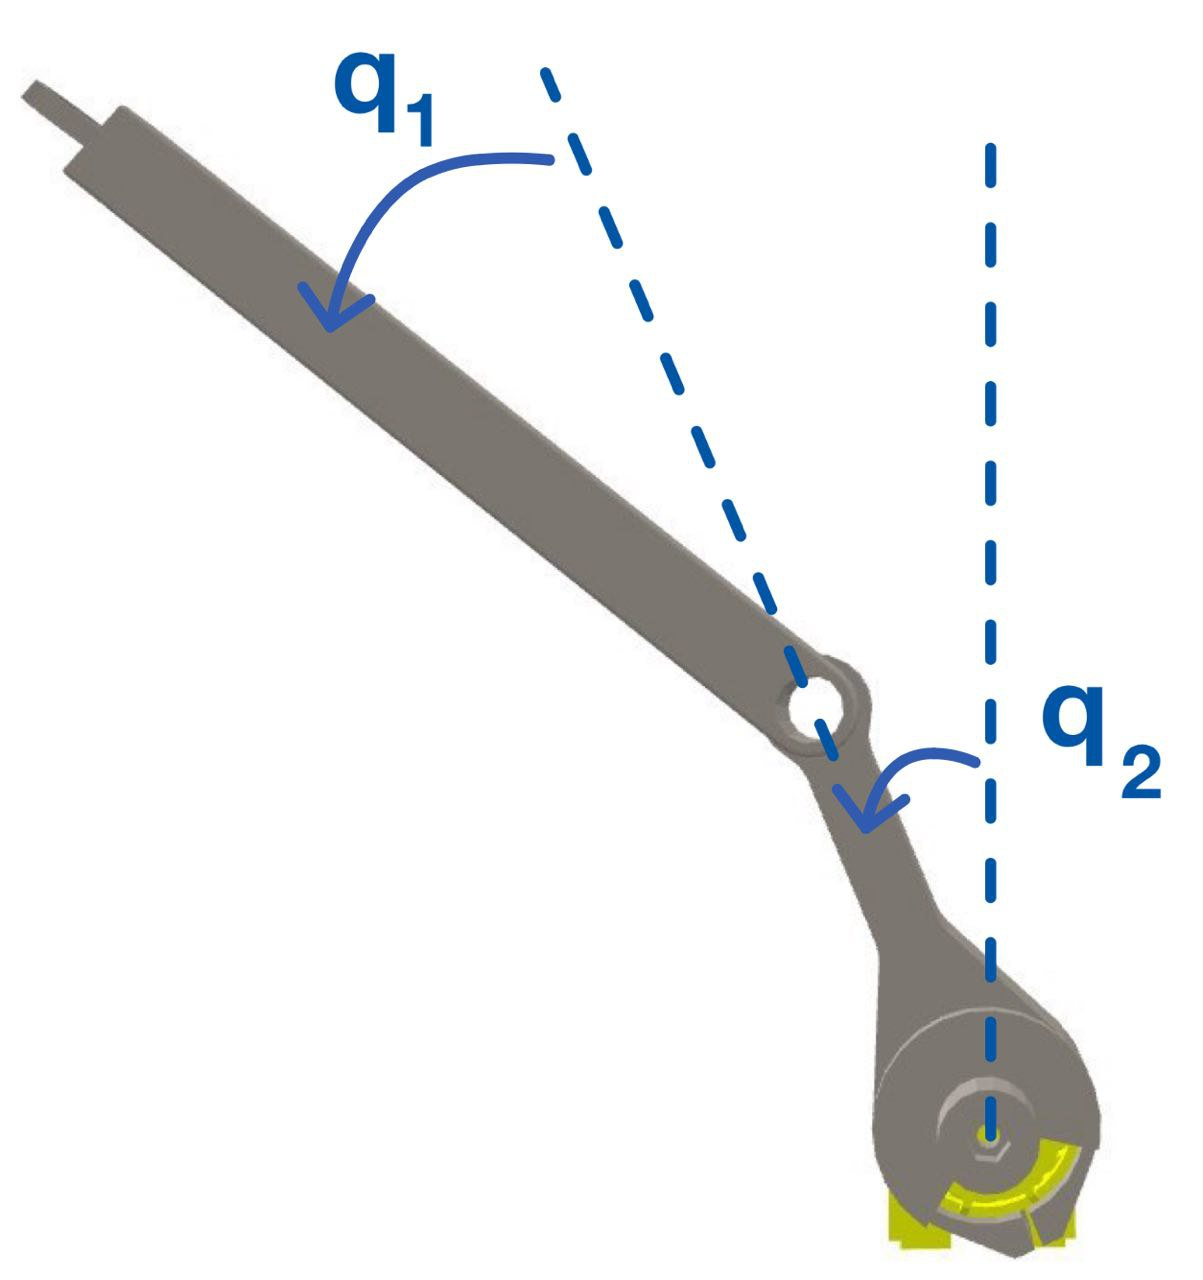
\includegraphics[width=0.3\textwidth]{pics/pend_q.jpg} 
    \caption{Double pendulum coordinates.}
    \label{fig:pend_q}
\end{figure}

\noindent Using the notation in Figure \ref{fig:pend_q}, the state of the system was defined as \(\mathbf{x} = [q_1, q_2, \dot{q_1}, \dot{q_2}]^T\). Where \(q_1\) and \(q_2\) are the angles, while \(\dot{q_1}\) and \(\dot{q_2}\) are the angular velocities of the first and second links, respectively. The control input was defined as the torque \(\mathbf{u} = \tau_1\) applied to the first joint, at the second joint, as previously mentioned, no torque is applied (\(\tau_2 = 0\)).\\

\noindent The OCP problem was defined as follows:

\vspace{-0.4cm}
\begin{equation}
\label{eq:ocp}
\begin{aligned}
    \min_{\mathbf{X}, \mathbf{U}} \quad & \sum_{k=0}^{N-1} \left( (\mathbf{x}_k - \mathbf{x}_{targ})^\top \mathbf{W}_x (\mathbf{x}_k - \mathbf{x}_{targ}) + (u_k - u_{targ})^\top \mathbf{W}_u (u_k - u_{targ}) \right) \\
    \text{subject to} \quad & \mathbf{x}_0 = \mathbf{x}_{init} \\
    & \mathbf{x}_{k+1} = \mathbf{f}(\mathbf{x}_k, u_k), \quad k = 0, \dots, N-1
\end{aligned}
\end{equation}

\noindent Where:
\begin{itemize}[noitemsep]
    \item $\mathbf{x}_{targ} = [0, 0, 0, 0]^\top$ is the target state.
    \item $\mathbf{u}_{targ} = [0]$ is the reference control input at equilibrium.
    \item $\mathbf{W}_x = \text{diag}(4e^0, 4e^0, 5e^{-1}, 1e^{-2})$ is the state weight matrix.
    \item $\mathbf{W}_u = [1e^0]$ is the control weight matrix.
    \item $\mathbf{x}_{init}$ is the initial state, which varies for each value in the dataset.
    \item $\mathbf{f}(\mathbf{x}_k, u_k)$ represents the system dynamics. 
\end{itemize}

\noindent Thus, the OCP cost was defined, within the CasADi framework, as a quadratic cost, penalizing the distance from the upright position, velocities, and the use of control input. The weights are chosen to allow the solver to find a solution in most initial conditions and to obtain physically reasonable motions.

It was later found that the cost defined in \eqref{eq:ocp} was not the most suitable for this problem, but this aspect will be discussed in the next sections.\\


\noindent The system's dynamics were modeled using the ADAM (\texttt{from adam.casadi}) library, which allows to compute the dynamics (thus the mass matrix $M(\mathbf{q})$ and bias forces $h(\mathbf{q}, \dot{\mathbf{q}})$) directly from the robot's URDF file. ($\mathbf{q} = [q_1, q_2]^\top$ are the joint angles vector).\\


\noindent This permits to solve the manipulator equation and find the joint accelerations $\ddot{\mathbf{q}} = \mathbf{M}(\mathbf{q})^{-1} (\boldsymbol{\tau} - \mathbf{h}(\mathbf{q}, \dot{\mathbf{q}}))$, where $\boldsymbol{\tau} = [\tau_1, 0]^\top$ accounts for the system's under-actuation. These accelerations were concatenated with the joint velocities $\dot{\mathbf{q}}$ to form the state derivative $\dot{\mathbf{x}} = [\dot{{q_1}}, \dot{q_2}, \ddot{{q_1}}, \ddot{{q_2}}]^\top$. Finally, the discrete-time state transition is achieved via an explicit Euler integration scheme, defined as $\mathbf{x}_{k+1} = \mathbf{x}_k + \dot{\mathbf{x}}_k \Delta t$, which maps the current state to the next over the time step $\Delta t$. 
So the function $\mathbf{f}(\mathbf{x}_k, u_k)$ in \eqref{eq:ocp} was defined as:
\begin{equation}
    \mathbf{f}(\mathbf{x}_k, u_k) = \mathbf{x}_k + \dot{\mathbf{x}}_k \Delta t  \  = \begin{bmatrix} \mathbf{q} \\ \dot{\mathbf{q}} \end{bmatrix}_{k} + \begin{bmatrix} \dot{\mathbf{q}} \\ \ddot{\mathbf{q}} \end{bmatrix}_{k} \cdot \Delta t
\end{equation}

%\noindent This was implemented as a CasADi function to be used inside the OCP solver.\\ Dico appena sopra che in OCP uso Casadi, quindi non serve ripeterlo

\noindent The following parameters were chosen for the OCP solver:
\begin{itemize}[noitemsep]
    \item Number of discretization steps: $N = 100$ steps
    \item Time step: $\Delta t = 0.05$ s
\end{itemize}

\noindent With all of this set up, the OCP problem in \eqref{eq:ocp} was solved 10.000 times, each with a different initial condition $\mathbf{x}_{init}$. At every run the initial state and the obtained cost were saved to generate the dataset. The initial conditions were sampled randomly from a uniform distribution within the following ranges:

\begin{itemize}[noitemsep]
    \item Joint 1 position ($q_1$): sampled from a uniform distribution in the range $[-\pi, \pi]$ rad.
    \item Joint 2 position ($q_2$): sampled from a uniform distribution in the range $[-0.9\pi, 0.9\pi]$ rad.
    \item Joint 1 velocity ($\dot{q}_1$): sampled from a uniform distribution in the range $[-8.0, 8.0]$ rad/s.
    \item Joint 2 velocity ($\dot{q}_2$): sampled from a uniform distribution in the range $[-15.0, 15.0]$ rad/s.
\end{itemize}

\noindent The ranges were selected to cover a broad spectrum of initial conditions, ensuring that the dataset captures a diversity of trajectories necessary to training the neural network. Simultaneously, the boundaries are set not to be too broad, in order to ensure that the state space remains sufficiently explored, maintaining a high density of samples within the region of interest to facilitate effective learning.

The samples of $q_2$ are limited to a value of $90\%$ of $\pi$ to avoid singularities in the dynamics computation when the second link is fully inverted.

The multiprocessing library of Python was also used, to parallelize the OCP solving process, speeding up the dataset generation.

\noindent An example of the motion obtained by solving the OCP from different initial conditions is shown in the video at the following link: \url{https://youtu.be/N8cDjysMnIY}. 

\noindent The initial conditions were: 

\begin{itemize}[noitemsep]
    \item Example 1: $\mathbf{x}_{init} = [2.88, 0.89, -10.0, -10.0]^\top$
    \item Example 2: $\mathbf{x}_{init} = [2.88, -0.89, 0.0, 0.0]^\top$
    \item Example 3: $\mathbf{x}_{init} = [0.47, -0.47, 0.0, 1.5]^\top$
    \item Example 4: $\mathbf{x}_{init} = [-1.2, 0.14, 1.65, 0.53]^\top$
\end{itemize}

%\noindent The motion obtained are shown in the video  at the following link: \url{https://youtu.be/N8cDjysMnIY}.
\newpage 
\noindent Finally, in the following Figure \ref{fig:run_dataset}, the dataset generation is reported:

\begin{figure}[H]
    \centering
    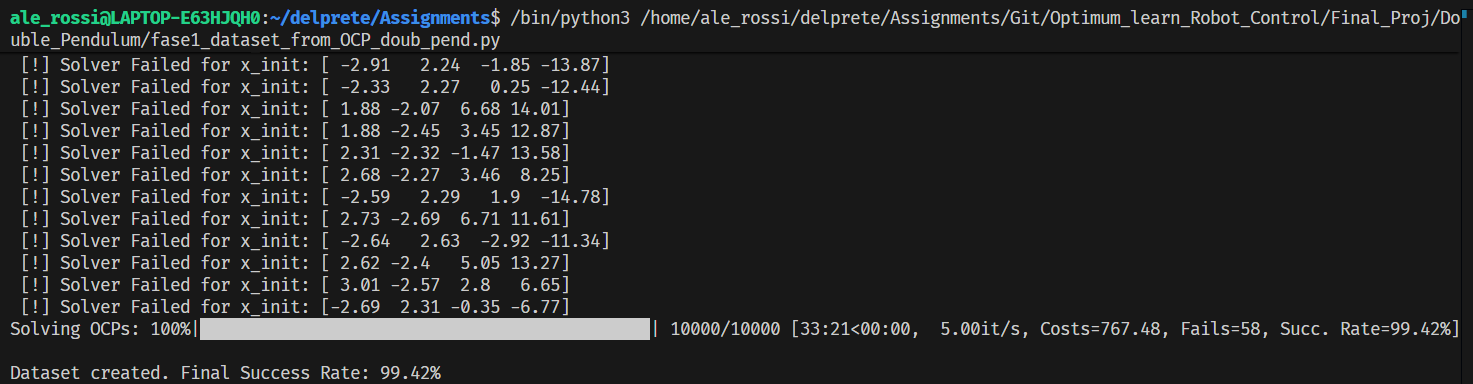
\includegraphics[width=0.9\textwidth]{pics/run_dataset.png} 
    \caption{Dataset generation results.}
    \label{fig:run_dataset}
\end{figure}

\noindent As can be seen, the solver has a success rate of $99.42\%$, meaning that $9942$ trajectories were successfully computed out of the $10000$ initial conditions sampled. The time to perform the whole dataset generation was $32.21$ minutes using $8$ parallel processes.

\noindent
Afterwards, the dataset is saved as a .npz file called \texttt{pendulum\_dataset\_used.npz}, containing two arrays: \texttt{inputs} of shape $(9942, 4)$ reporting the initial states and \texttt{targets} of shape $(9942, 1)$ illustrating the corresponding costs. The dimension is not 10000 because some trajectories failed to be computed by the solver.\\

\noindent All of this was implemented in the file: "\texttt{fase1\_dataset\_from\_OCP\_doub\_pend.py}"
\\

\noindent The content of the dataset was then visualized using a Parallel Coordinates Plot, shown in Figure \ref{fig:cost_dataset}:

\begin{figure}[H]
    \centering
    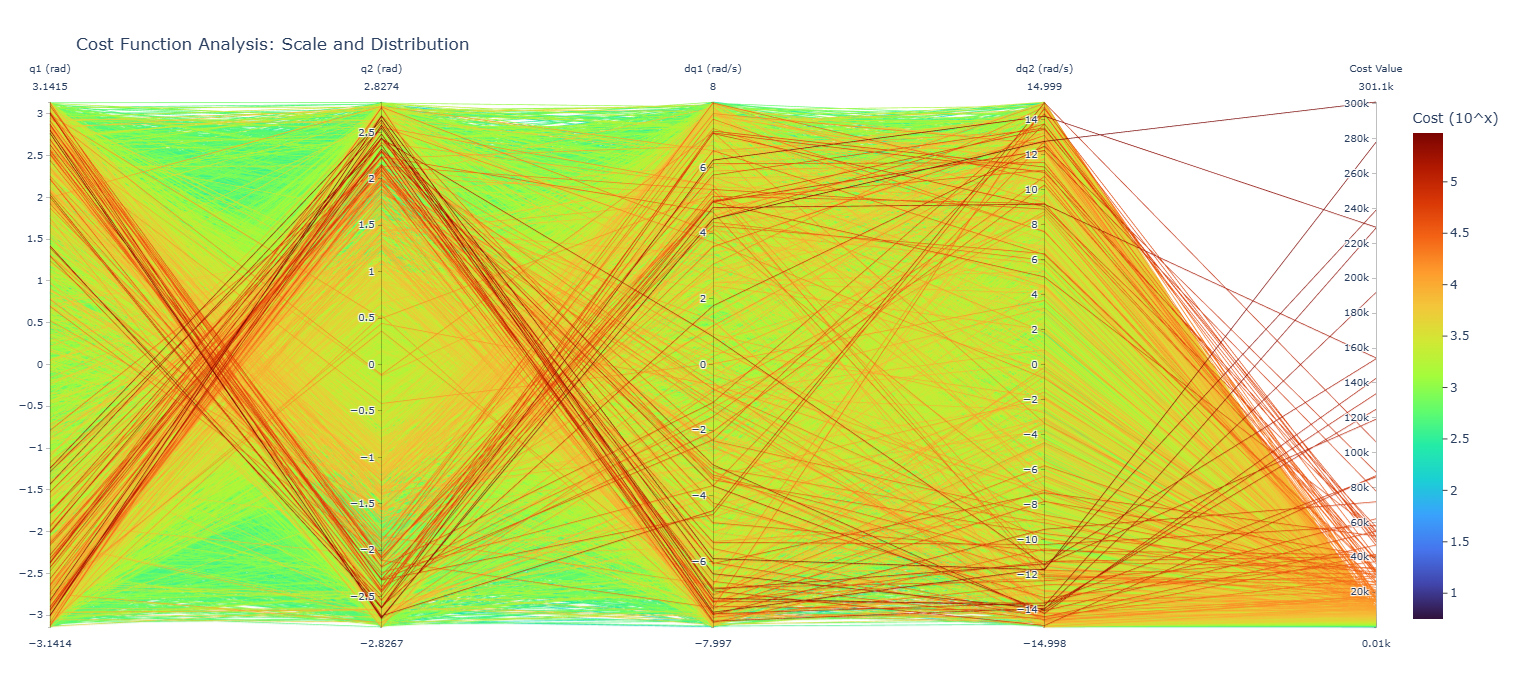
\includegraphics[width=0.9\textwidth]{pics/cost_dataset.png} 
    \caption{Parallel Coordinates Plot of the dataset.}
    \label{fig:cost_dataset}
\end{figure}

\noindent From the plot, it can be observed that the cost values span several orders of magnitude, ranging from approximately $10^0$ to $10^5$. This wide range indicates that some initial conditions lead to significantly higher costs than others. However the vast majority of the values are under $20\ 000$. For this reason we considered the values above this number as outliers and we decided to remove them from the dataset before training the neural network. This choice was made to prevent these extreme values from skewing the training process and adversely affecting the model's performance on more typical scenarios. (To interact with the plot, please run the \texttt{dataset\_cost\_plot.py} file).